\begin{center}
    \textbf{BAB III} \\[0.5em]
    \textbf{METODE PENELITIAN}
\end{center}

\subsection*{3.1 Pengertian Metodologi Penulisan}
\textbf{Pengertian Metodologi Penulisan}

Metodologi penulisan merupakan bagian dari ilmu pengetahuan yang mempelajari bagaimana prosedur kerja mencari kebenaran (Muhajir, 2000). Metodologi adalah awal dari metode dan lebih mendasar dibandingkan metode. Metodologi menyediakan dasar-dasar kerja filosofis bagi sebuah metode (Kuswarno, 2009).

Metode penulisan mengacu pada prosedur tertentu untuk mengumpulkan dan menganalisis data (Wilis, 2007). Metode untuk penulisan kuantitatif berbeda dengan penulisan kualitatif. Penulisan kualitatif adalah jenis penulisan yang menghasilkan penemuan-penemuan yang tidak dapat diperoleh dengan menggunakan prosedur statistik atau cara-cara lain dari kuantifikasi (Creswell, 2007). Metode penulisan merupakan cara ilmiah untuk mendapatkan data dengan tujuan dan kegunaan tertentu (Sugiyono, 2017, 3). Cara ilmiah berarti penulisan didasarkan pada ciri-ciri keilmuan yaitu:
\begin{itemize}
    \item Rasional, artinya penulisan dilakukan dengan cara yang masuk akal.
    \item Empiris, artinya cara-cara yang digunakan dapat diamati.
    \item Sistematis, artinya penulisan menggunakan langkah-langkah tertentu yang bersifat logis.
\end{itemize}

\subsection*{3.2 Metodologi Pengembangan Sistem}
Metodologi yang digunakan dalam pengembangan sistem aplikasi \textit{task tracker} berbasis web ini adalah \textit{Agile Methodology}. \textit{Agile} merupakan pendekatan pengembangan perangkat lunak yang bersifat iteratif dan inkremental, serta menekankan kolaborasi, fleksibilitas, dan adaptasi terhadap perubahan kebutuhan pengguna.

Metodologi ini terdiri atas beberapa tahapan:
\begin{enumerate}
    \item \textbf{Requirement Gathering} (Pengumpulan Kebutuhan)
    \newline Pada tahap ini dilakukan identifikasi kebutuhan sistem aplikasi \textit{task tracker} berdasarkan permasalahan yang ingin diselesaikan, yaitu manusia sering kali dihadapkan pada berbagai aktivitas dan tanggung jawab yang harus diselesaikan dalam waktu tertentu. 
    Namun, tidak jarang kita lupa apa yang sudah dikerjakan sebelumnya, atau bingung menentukan apa yang harus dilakukan selanjutnya. 
    Hal ini bisa menyebabkan penurunan produktivitas, ketidakteraturan, dan bahkan stres akibat pekerjaan yang menumpuk tanpa perencanaan.
    \newline Untuk mengatasi permasalahan tersebut, dibutuhkan sebuah sistem yang dapat membantu individu dalam mencatat, mengelola, dan melacak kegiatan sehari-hari secara terstruktur.
    Aplikasi \textit{task tracker} hadir sebagai solusi praktis untuk mencatat aktivitas harian, mengingatkan tugas yang belum selesai, dan memberikan gambaran yang jelas mengenai progres harian maupun mingguan pengguna.
    \item \textbf{Design} (Perancangan)
    Desain dilakukan secara bertahap dan langsung mendukung fitur yang akan dikembangkan. Karena pengerjaan dilakukan secara mandiri dan tidak formal, desain difokuskan pada: Struktur basis data menggunakan PostgreSQL. Arsitektur MVC dengan Laravel (PHP webframework). 
    Desain antarmuka yang sederhana dan fungsional, berfokus pada penggunaan harian.
    \item \textbf{Development} (Pengembangan/Koding)
    Setelah Pada tahap ini dilakukan implementasi kode sesuai dengan fitur yang direncanakan.
    Proses pengembangan dilakukan secara iteratif, satu fitur pada satu waktu, seperti:
    \begin{itemize}
        \item Pengerjaan fitur login dan registrasi
        \item Pengerjaan fitur workspace management
        \item Pengerjaan fitur task management
    \end{itemize}
    \item \textbf{Testing} (Pengujian)
    Pada tahap ini Setelah fitur dikembangkan, dilakukan pengujian fungsional secara manual seperti: 
    \begin{itemize}
        \item Integration Testing: Memastikan setiap bagian sistem saling terhubung dengan baik (contoh: form input tugas terhubung ke tampilan list).
        \item System Testing: Pengujian keseluruhan aplikasi melalui skenario penggunaan sehari-hari.
        \item User Acceptance Testing: Pengujian dilakukan oleh pengembang sendiri sebagai pengguna utama.
    \end{itemize}
    \item \textbf{Deployment} (Penerapan)
    Pada tahapan ini aplikasi kemudian dijalankan di lingkungan produksi lokal atau server pribadi.
    \item \textbf{Review} (Maintenance/Pemeliharaan)
    Tahap ini mencakup perbaikan bug yang ditemukan selama penggunaan, serta penambahan fitur baru berdasarkan pengalaman pribadi.
    Proses review dilakukan secara berkala: Menyempurnakan tampilan antarmuka.
    Mengoptimalkan proses pengambilan data. 
    Menambahkan fitur tambahan jika perlu
\end{enumerate}


\subsection*{3.3 Tujuan Project}
\begin{itemize}
    \item Membantu pengguna mencatat dan merencanakan aktivitas harian agar tidak ada tugas yang terlewat. 
    \item Meningkatkan produktivitas dengan pengelolaan waktu dan tugas yang lebih terorganisir.
    \item Mempermudah proses tracking kegiatan harian untuk refleksi dan evaluasi diri.
    \item Membantu pengguna membangun kebiasaan yang konsisten dalam menyelesaikan tugas-tugasnya. 
    \item Memberikan antarmuka yang sederhana dan mudah digunakan, sehingga bisa digunakan oleh siapa saja dalam berbagai aktivitas sehari-hari. 
    \item Menyediakan fitur workspace agar pengguna dapat mengelola aktivitas dalam konteks kerja sama tim atau proyek tertentu.
\end{itemize}

\subsection*{3.4 Batasan Projek Task Tracker}
\begin{itemize}
    \item User Management
    fitur ini mencakup fitur registrasi dan login user, sehingga data pada website bisa terhubung sesuai dengan user yang sedang login.
    website juga mempunyai menu profile sehingga user bisa mengupdate nama user dan password jika dibutuhkan
    \item Wokspace Management
    Fitur workspace berguna agar user bisa 
    \item Task Management
    \item Task Board
    \item Dashboard  
\end{itemize}

\subsection*{3.5 Usecase Diagram}
\begin{itemize}
  \item User Management
  \newline
  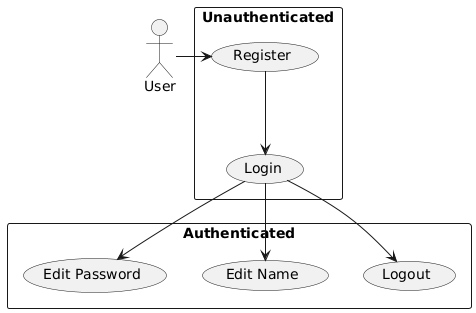
\includegraphics[width=0.4\textwidth]{assets/usecase_diagrams/auth.png}
  \item Workspace Management
  \newline
  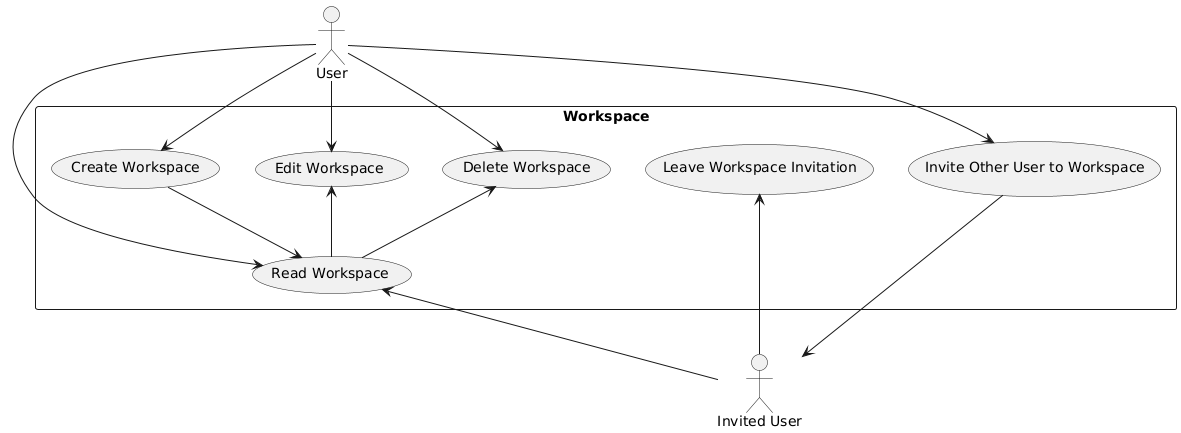
\includegraphics[width=0.4\textwidth]{assets/usecase_diagrams/workspace.png}
  \item Task Management
  \newline
  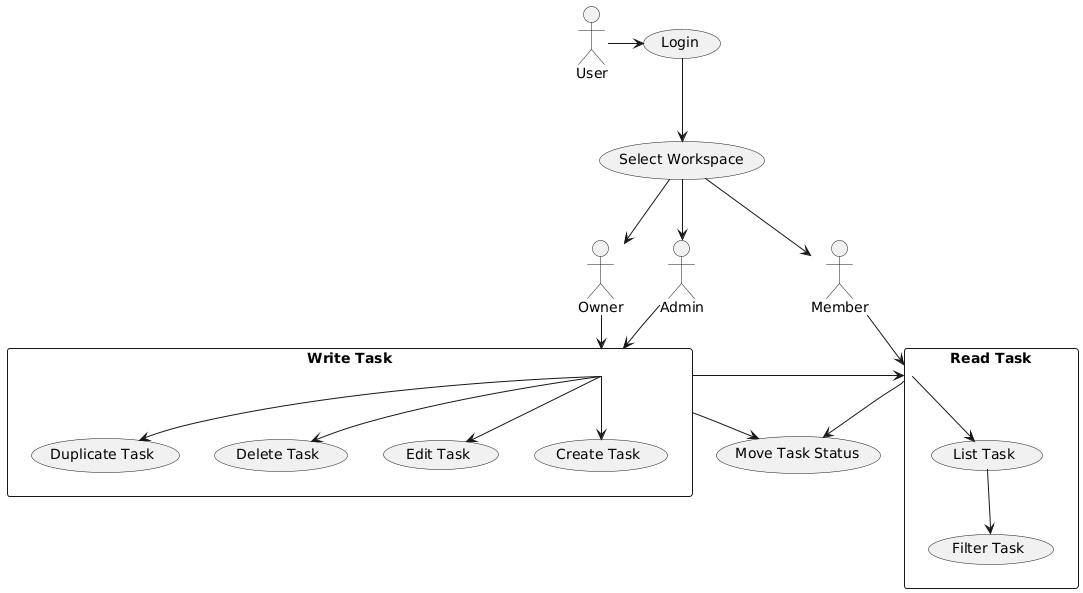
\includegraphics[width=0.5\textwidth]{assets/usecase_diagrams/task.png}
\end{itemize}

\subsection*{3.6 Class Diagram}
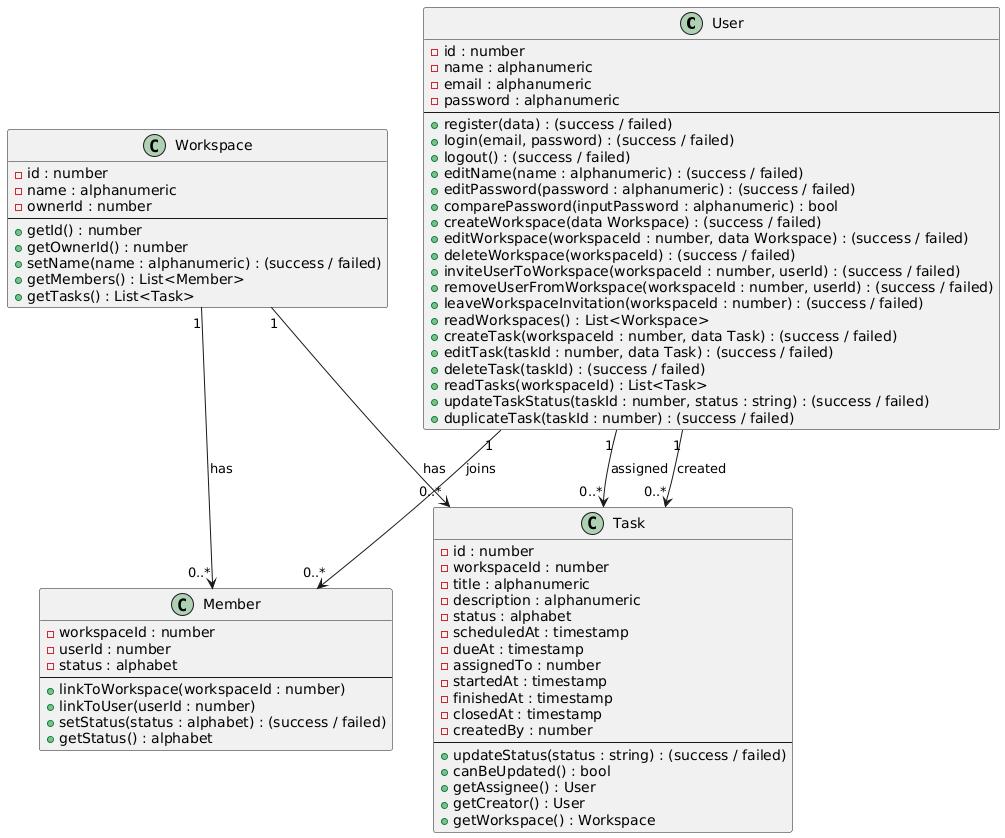
\includegraphics[width=1\textwidth]{assets/class_diagram.png}

\subsection*{3.7 Activity Diagram}
                                 
\begin{itemize}
  \item User Login
  \newline
  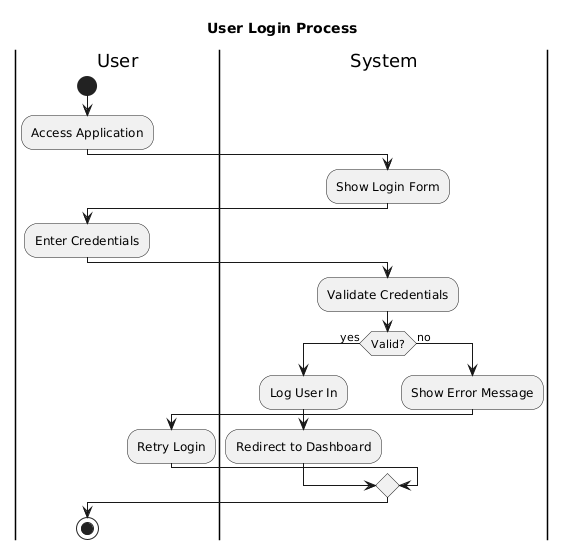
\includegraphics[width=0.4\textwidth]{assets/activity_diagrams/user_login.png}
  \item User Logout
  \newline
  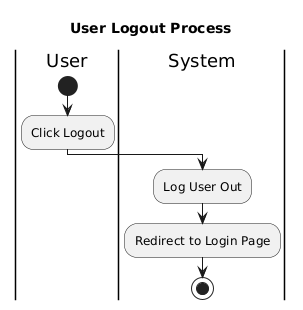
\includegraphics[width=0.4\textwidth]{assets/activity_diagrams/user_logout.png}
  \item User Profile Update Name
  \newline
  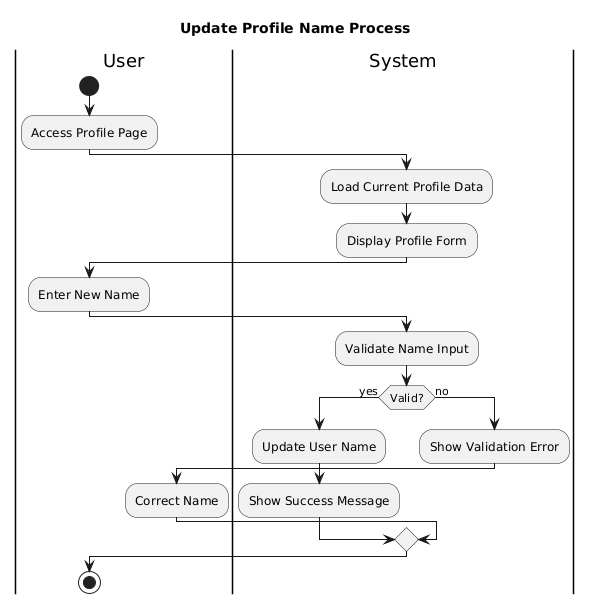
\includegraphics[width=0.4\textwidth]{assets/activity_diagrams/user_profile_update_name.png}
  \item User Profile Update Password
  \newline
  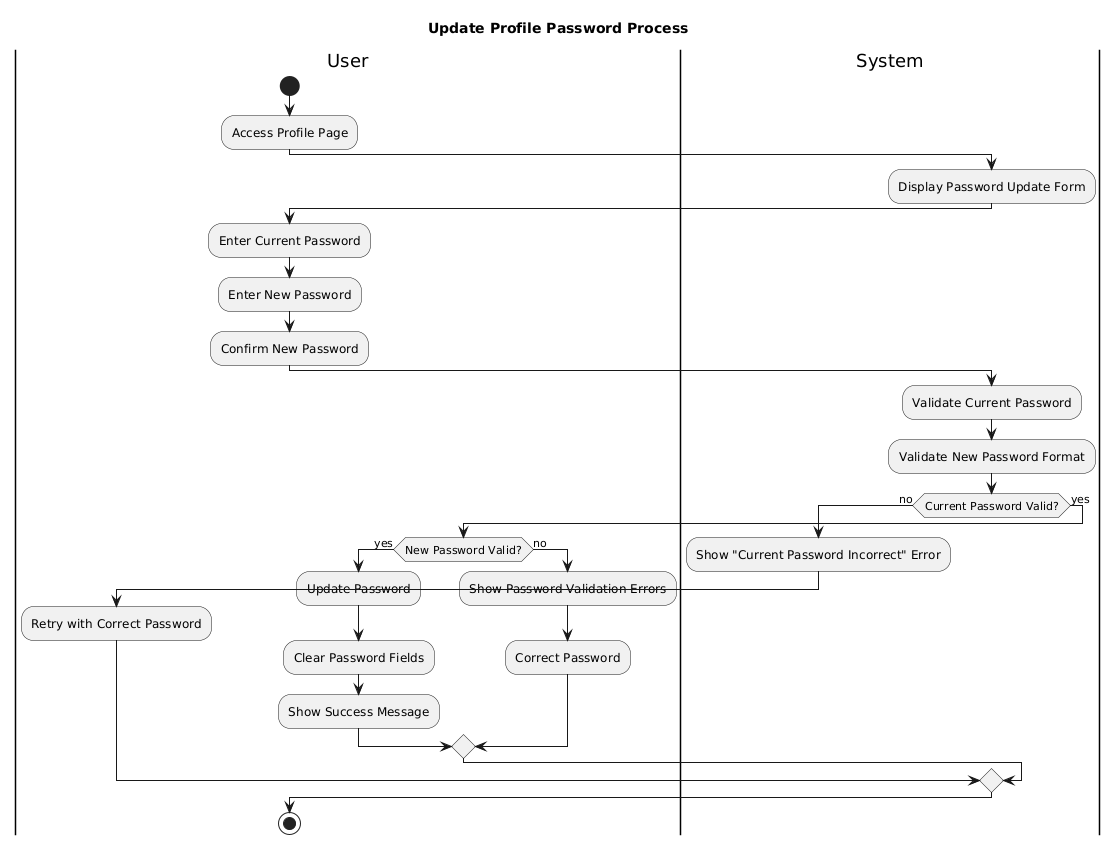
\includegraphics[width=0.4\textwidth]{assets/activity_diagrams/user_profile_update_password.png}
  \item Workspace Create
  \newline
  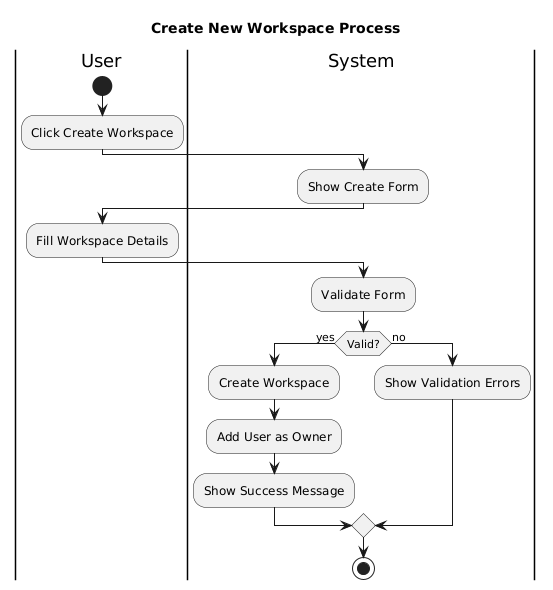
\includegraphics[width=0.4\textwidth]{assets/activity_diagrams/workspace_create.png}
  \item Workspace Update
  \newline
  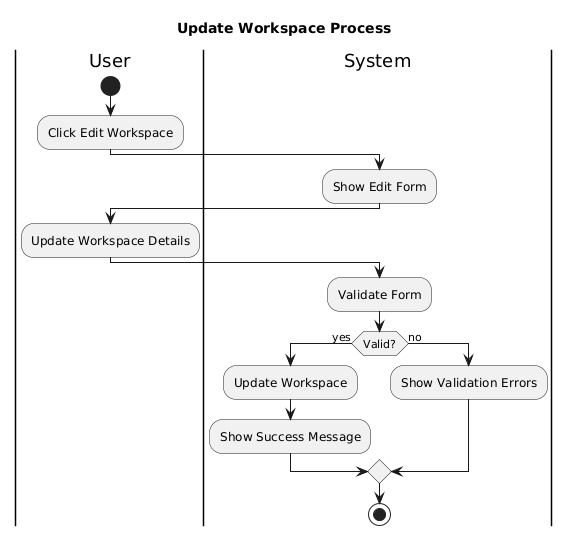
\includegraphics[width=0.4\textwidth]{assets/activity_diagrams/workspace_update.png}
  \item Workspace Invite
  \newline
  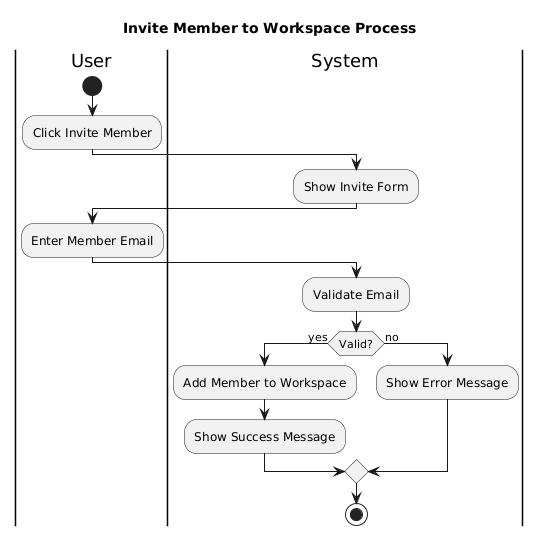
\includegraphics[width=0.4\textwidth]{assets/activity_diagrams/workspace_invite.png}
  \item Workspace Remove
  \newline
  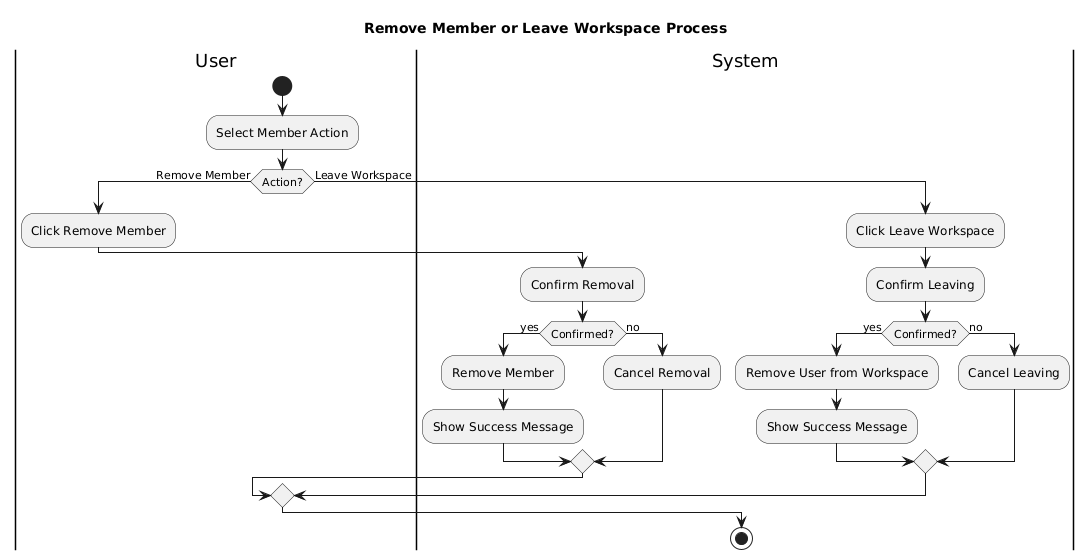
\includegraphics[width=0.8\textwidth]{assets/activity_diagrams/workspace_remove.png}
  \item Workspace Delete
  \newline
  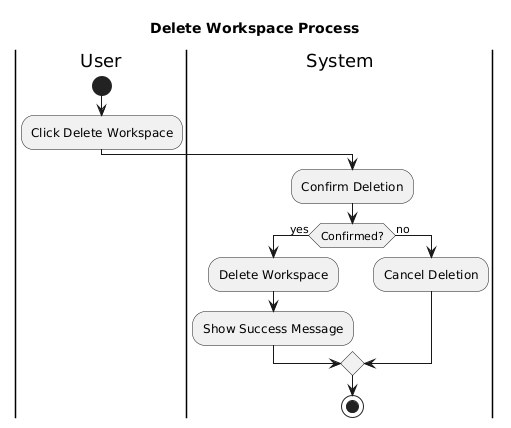
\includegraphics[width=0.4\textwidth]{assets/activity_diagrams/workspace_delete.png}
  \item Task Create
  \newline
  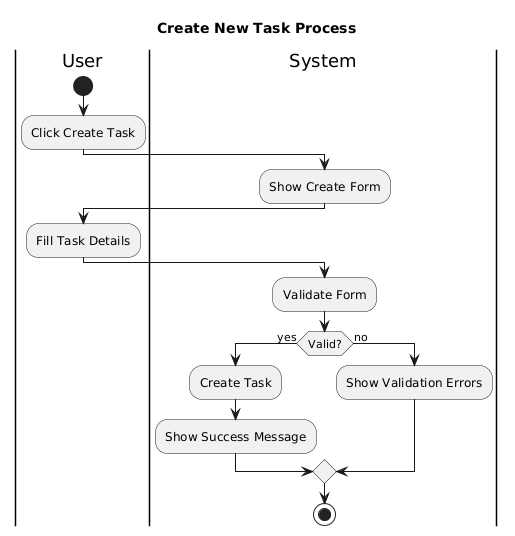
\includegraphics[width=0.4\textwidth]{assets/activity_diagrams/task_create.png}
  \item Task Read
  \newline
  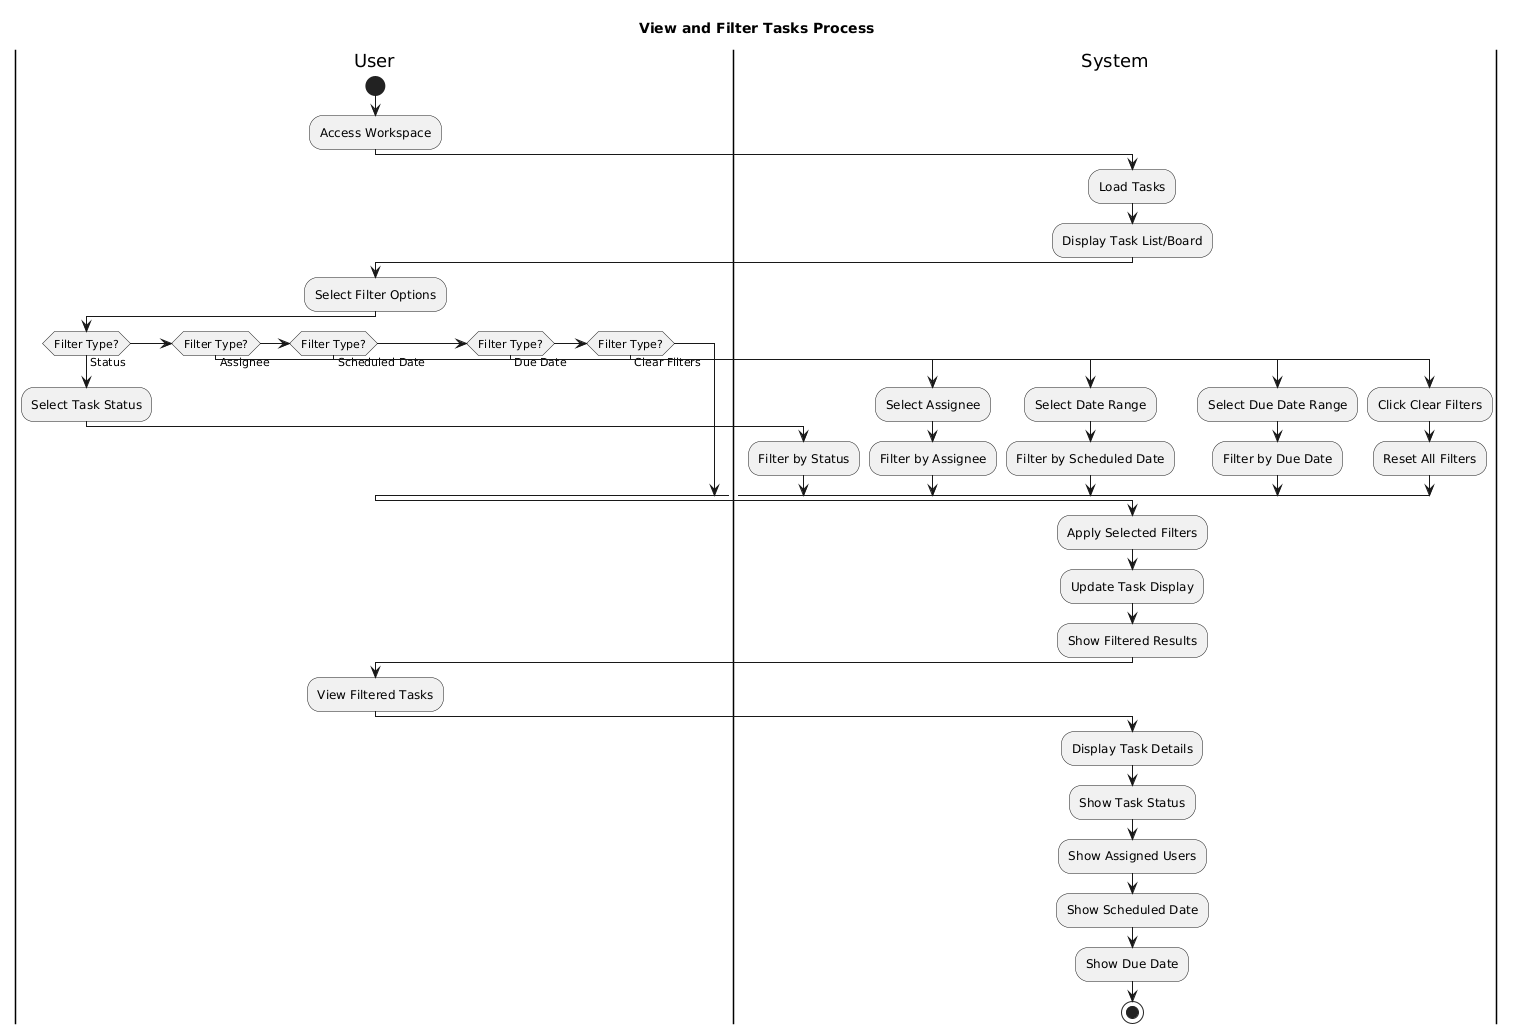
\includegraphics[width=0.8\textwidth]{assets/activity_diagrams/task_read.png}
  \item Task Update
  \newline
  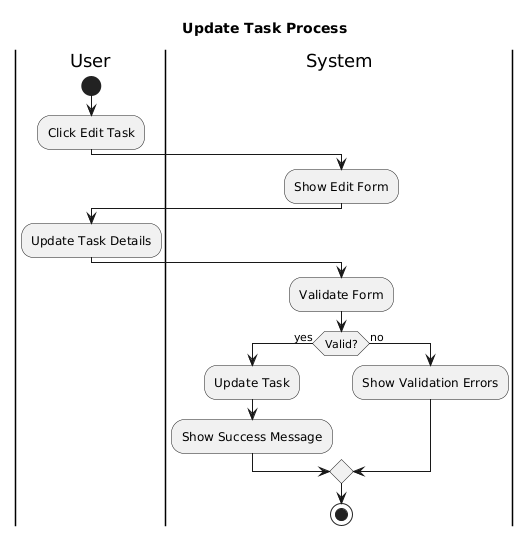
\includegraphics[width=0.4\textwidth]{assets/activity_diagrams/task_update.png}
  \item Task Delete
  \newline
  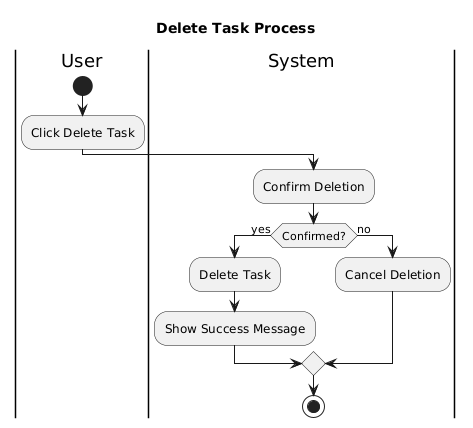
\includegraphics[width=0.4\textwidth]{assets/activity_diagrams/task_delete.png}
  \item Task Duplicate
  \newline
  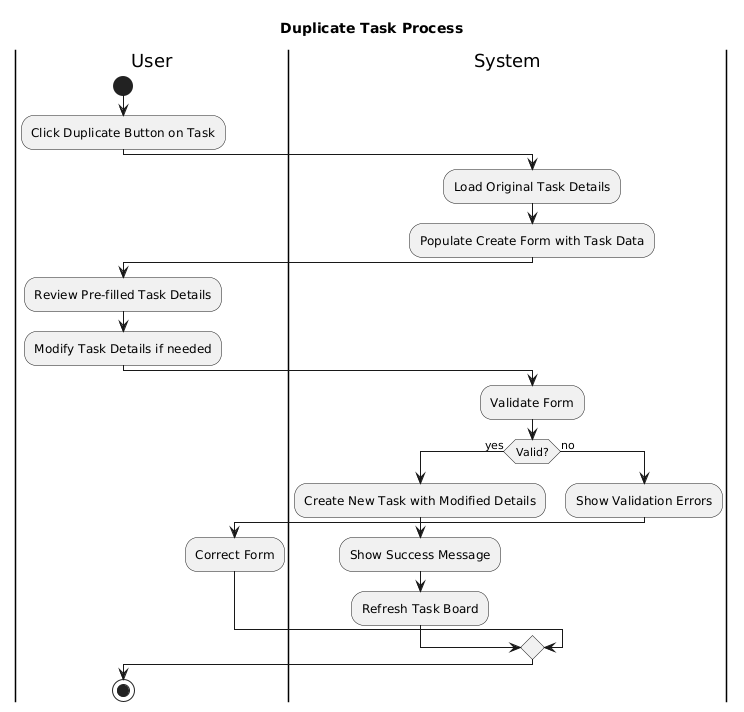
\includegraphics[width=0.4\textwidth]{assets/activity_diagrams/task_duplicate.png}
\end{itemize}